

%\documentclass[9pt]{beamer}

\documentclass[usenames,dvipsnames, xcolor=table, 9pt]{beamer}
\usepackage{spot}
\usepackage{graphicx}

%\usepackage[ruled,vlined]{algorithm2e}
\usepackage{algorithm, algorithmic}
%\usepackage[table]{xcolor}
\usepackage{color,soul}
\usepackage[utf8]{inputenc}
\usepackage{geometry}
\geometry{textwidth=7cm}
\usepackage{amsmath}
\usepackage{cancel}
\usepackage{amsmath}
\usepackage{spot}
\usepackage{graphicx} % Allows to include images
\usepackage{booktabs} % Allows the use of \toprule, \midrule and \bottomrule in tables
\usepackage[labelformat=empty]{caption}
\usepackage{times}
\usepackage{graphicx,epsfig,psfrag,float,color}
\usepackage{tikz}
\usepackage{pgfplots}
\pgfplotsset{compat=1.15}
\usepackage{multirow}

\usepackage{setspace}
\usepackage[first=0,last=9]{lcg}
\usepackage{amsmath}
\definecolor{Gray}{gray}{0.9}


\usepackage{ragged2e}
\usepackage{appendixnumberbeamer}


\usepackage{hyperref}
%\hypersetup{colorlinks,linkcolor=blue,urlcolor=blue}

%\definecolor{yell}{yellow}{0.9}

\newcolumntype{g}{>{\columncolor{lime}}c}

\newcolumntype{w}{>{\columncolor{white}}c}
\newcommand{\ra}{\rand0.\arabic{rand}}


\DeclareMathOperator{\SP}{SP}
\DeclareMathOperator{\relu}{ReLU}
\DeclareMathOperator{\alter}{alter}
\DeclareMathOperator{\feat}{feat}
\DeclareMathOperator{\sign}{sign} 
\DeclareMathOperator{\simi}{sim}
\usepackage{array}

\definecolor{olive}{rgb}{0.3, 0.4, .1}
\definecolor{fore}{RGB}{249,242,215}
\definecolor{back}{RGB}{51,51,51}
\definecolor{title}{RGB}{255,0,90}
\definecolor{dgreen}{rgb}{0.,0.6,0.}
\definecolor{gold}{rgb}{1.,0.84,0.}
\definecolor{JungleGreen}{cmyk}{0.99,0,0.52,0}
\definecolor{BlueGreen}{cmyk}{0.85,0,0.33,0}
\definecolor{RawSienna}{cmyk}{0,0.72,1,0.45}
\definecolor{Magenta}{cmyk}{0,1,0,0}
\definecolor{armygreen}{rgb}{0.29, 0.33, 0.13}


\DeclareMathOperator{\n2v}{node2vec}

\newcommand\Tstrut{\rule{0pt}{2.08 ex}} 
\newcommand\Bstrut{\rule[-0.9ex]{0pt}{0pt}}


\setbeamertemplate{bibliography item}{\insertbiblabel}


%\logo{%
  %\makebox[0.95\paperwidth]{%
   %\includegraphics[width=1.6cm,keepaspectratio]{Figures/Marca_IFSP_2015_Araraquara-05.png}
    %\hfill%
    %\includegraphics[width=0.17\paperwidth]{fim3.png}%
  %}%
%\vspace{235pt}
%}


\mode<presentation> {

\usetheme{default}
\definecolor{OISTcolor}{rgb}{0.65,0.16,0.16}

%\usecolortheme[named=OISTcolor]{structure} % Use this line for OIST colors
\usecolortheme[named=black]{structure} % Black titles and such

\setbeamertemplate{itemize item}{\color{black}$\bullet$} % Comment this line for default bullet points (colored triangles)

\usepackage{helvet} % Helvetica Font 
\renewcommand{\familydefault}{\sfdefault}

\setbeamertemplate{navigation symbols}{} % No navigation symbols
\setbeamertemplate{footline} % Only page number at the bottom
 {\begin{minipage}{125mm} \vspace{-3 mm} \hfill \insertframenumber \end{minipage}}
 }

\definecolor{UHGreen}{RGB}{0, 77, 0}
\definecolor{UHTeal}{RGB}{0,116,122}
\definecolor{UHBlue}{RGB}{0,35,149}
\definecolor{UHLtBlue}{RGB}{113,111,179}
\definecolor{UHBrown}{RGB}{179,153,93}
\definecolor{ao(english)}{rgb}{0.0, 0.5, 0.0}

\definecolor{amaranth}{rgb}{0.9, 0.17, 0.31}

\setbeamercolor{structure}{fg=UHGreen}
\setbeamercolor{title}{fg=black}
\setbeamerfont{structure}{series=\bfseries}
\setbeamerfont{title}{series=\bfseries}
\newcommand{\myRed}[1]{\textcolor{red}{#1}}

\setbeamerfont{block title alerted}{series=\bfseries}
\setbeamercolor{block title}{bg=UHBlue,fg=UHLtBlue!20!white}
\setbeamercolor{block body}{bg=UHLtBlue!15!white}
\setbeamercolor{block title example}{bg=UHBrown!60!white}
\setbeamercolor{block body example}{bg=UHBrown!20!white}
\setbeamercolor{block title alerted}{bg=red!60!white,fg=black}
\setbeamercolor{block body alerted}{bg=red!10!white}

\DeclareMathOperator{\KL}{KL}

\usepackage{textpos}

\makeatletter
\let\HL\hl
\renewcommand\hl{%
	\let\set@color\beamerorig@set@color
	\let\reset@color\beamerorig@reset@color
	\HL}
\makeatother

\newcommand*{\superscript}[1]{\ensuremath{^{\rm #1}}}
\newcommand*{\subscript}[1]{\ensuremath{_{\rm #1}}}

\renewcommand{\insertshorttitle}{{\fontsize{6pt}{6}\selectfont { Graph Embedding \& Social Networks}}}
\renewcommand{\insertshortauthor}{{\fontsize{6pt}{6}\selectfont {Fatemeh Salehi Rizi }}}
\newcommand{\address}{ }

\date{}

\setbeamertemplate{footline}{
   \begin{beamercolorbox}[ht=1ex,leftskip=1.2cm,rightskip=0.3cm]{}
   % ht: altura
   % \textcolor{black}{\hrule height 5pt}
   % \vspace{0.4cm}\insertshortauthor
     {\fontsize{6pt}{6}\selectfont {\insertsection}} \hfill  {\fontsize{6pt}{6}\selectfont {\insertframenumber/\inserttotalframenumber}}
   \end{beamercolorbox}
   \vspace*{0.178 cm}
} 


\newcommand{\backupbegin}{
	\newcounter{finalframe}
	\setcounter{finalframe}{\value{framenumber}}
}
\newcommand{\backupend}{
	\setcounter{framenumber}{\value{finalframe}}
}


\makeatletter
\newbox\@backgroundblock
\newenvironment{backgroundblock}[2]{%
  \global\setbox\@backgroundblock=\vbox\bgroup%
    \unvbox\@backgroundblock%
    \vbox to0pt\bgroup\vskip#2\hbox to0pt\bgroup\hskip#1\relax%
}{\egroup\egroup\egroup}
\addtobeamertemplate{background}{\box\@backgroundblock}{}
\makeatother

%----------------------------------------------------------------------------------------
%	TITLE PAGE
%----------------------------------------------------------------------------------------



\title[Short title]{\textcolor{UHGreen}{ Title of the talk ...}}

\author{Name} % Your name

%\address
 
%\date{March 29, 2023} % Date, leave empty, use subtitle instead



%\subtitle{ hhh}
%%%%%%%%%%%%%%%%%%%%%%%%%%%%%%%%%%%%%%%%%%%%%%%%%%%%%%%%%%%%%%%%%%%%%%%%%%%%%%%%%%%%%%%

\begin{document}
\setstretch{1.15}


	
\setbeamertemplate{background}{
\includegraphics[width=0.999\paperwidth, trim=0 0 0 -615]{pics/footer2}}	

	
\setbeamertemplate{background}{
\includegraphics[width=\paperwidth]{pics/title2.pdf}} % Adding the background logo for the title page


\begin{frame}[t, plain]
%\vspace{.3cm}


\vspace{2.4cm}
%\vspace*{1.55cm} % Use this spacing if author field is empty
%\vspace*{5mm}  % Use this spacing if author field is used
\titlepage % Print the title page as the first slide

\begin{center}
	Date
\end{center}
\end{frame}
%
\setbeamertemplate{background}{
\includegraphics[width=0.999\paperwidth, trim=0 0 0 -615]{pics/footer2}} % Adding the background logo for the rest of the slides trim=0 0 0 -900
%



\begin{frame}{Outline}
	
	
\begin{textblock*}{\paperwidth}(-0.17 \paperwidth, -30 mm)%
	\hfill 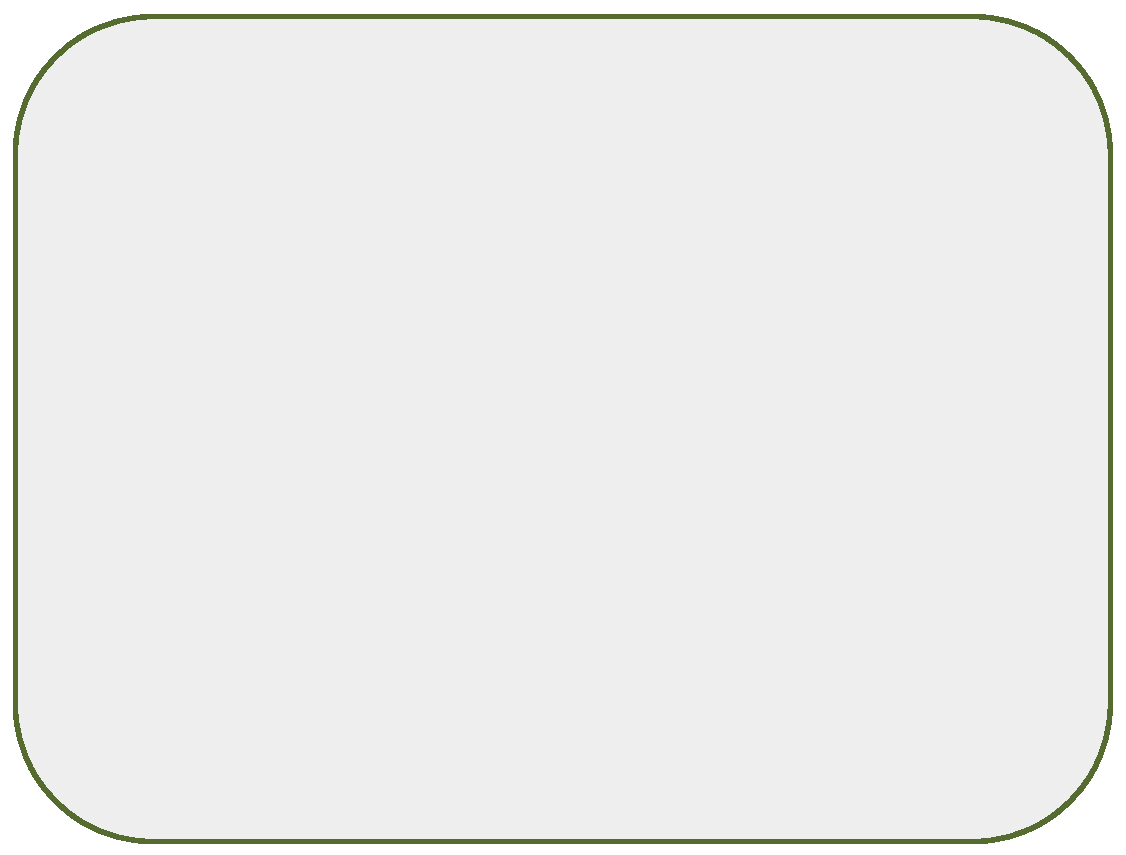
\includegraphics [width=0.81\linewidth ]{pics/bg_33}%
	
\end{textblock*}	


\begin{textblock*}{0.86\paperwidth}(0.06\paperwidth, -20 mm)%
	
	
	\begin{itemize}
	
		
		\item Introduction over
		\vspace{0.3 cm}
	
	
			
		\end{itemize}
	
	
\end{textblock*}
	
\end{frame}



\begin{frame}{Title ...}
	
	
	\begin{textblock*}{\paperwidth}(-0.14 \paperwidth, -29 mm)%
		
		\hfill 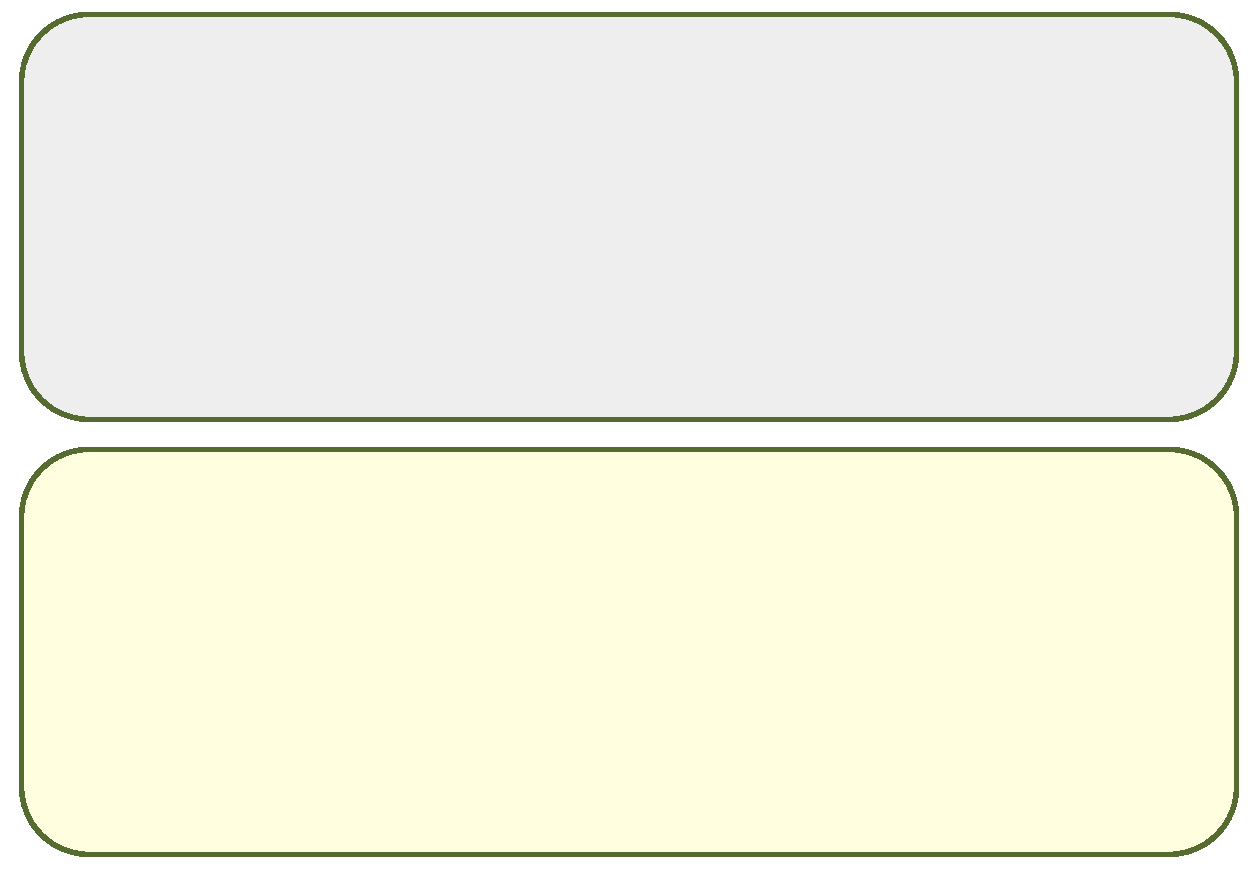
\includegraphics [width=0.85\paperwidth]{./pics/bckg01.pdf}
	\end{textblock*}
	
	\begin{textblock*}{0.8\paperwidth}(0.00 \paperwidth, -24mm)%
		\begin{itemize}
		\item[] Traditional Methods
		\vspace{0.3 cm}
		\small
		
		\begin{itemize}
			
		
			\item Distance-based
				\vspace{0.2 cm}
			\item Partition-based
				\vspace{0.2 cm}
		    \item Classification based
			
		\end{itemize}
	
\end{itemize}
		
	\end{textblock*}
	
	\begin{textblock*}{0.8\paperwidth}(0.00 \paperwidth, 15mm)%
		
		\begin{itemize}
			
			\item[] Deep Learning Methods 
			\vspace{0.3 cm}
			
			\begin{itemize}
				
			\item Reconstruction-based: 	Omni~\cite{omni}
				
					\vspace{0.32 cm}
						
			\item Prediction-based: 
			
	
			
			
		\end{itemize}	
			
	
			
		\end{itemize}
		
	\end{textblock*}
	
	
	
\end{frame}










\begin{frame}{Future Works}
	
	\begin{textblock*}{\paperwidth}(-0.18 \paperwidth, -30 mm)%
		\hfill 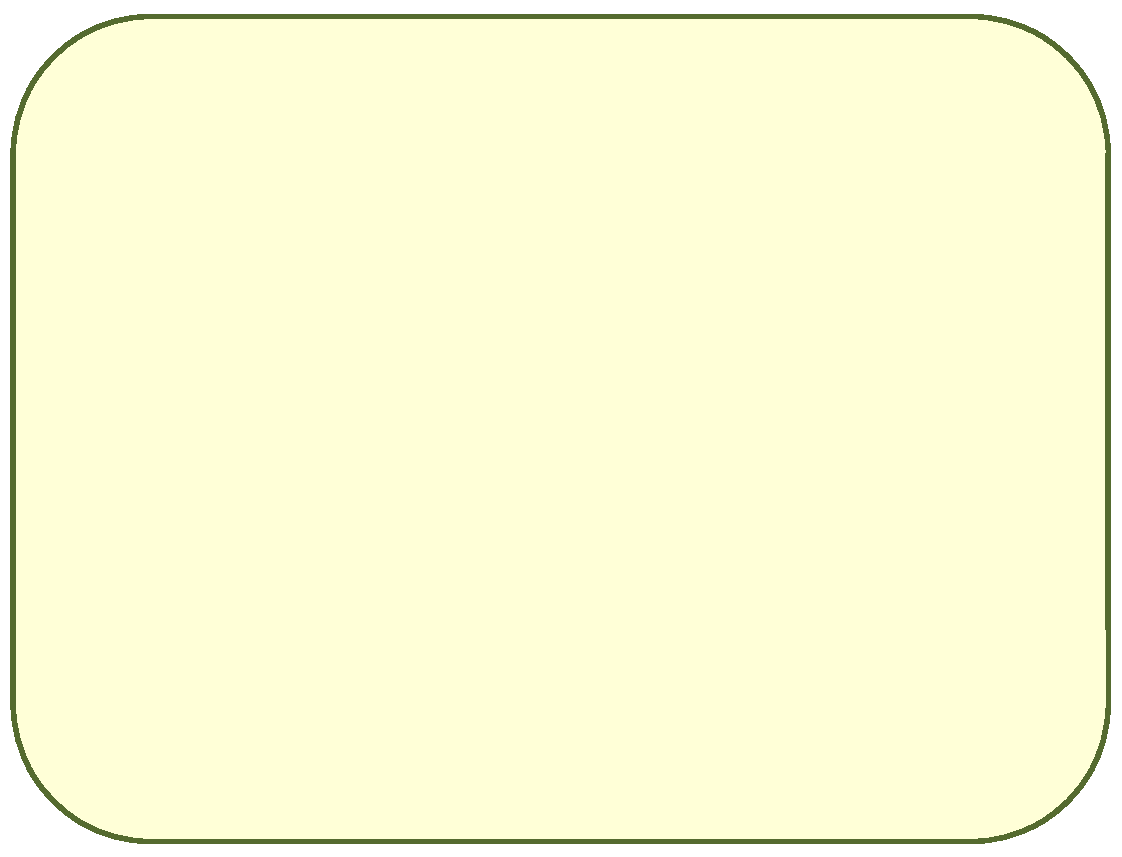
\includegraphics [width=0.8 \linewidth ]{pics/bg_99}%
		
	\end{textblock*}
	
	\begin{textblock*}{0.75\paperwidth}(0.05 \paperwidth, -20 mm)
		
		\begin{itemize}
		
			
			\item Traditional techniques 
			
	
		
			
		\end{itemize}
		
		
	\end{textblock*}

	
\end{frame}



\begin{frame}{Future Works}
	
	\begin{textblock*}{\paperwidth}(-0.18 \paperwidth, -30 mm)%
		\hfill 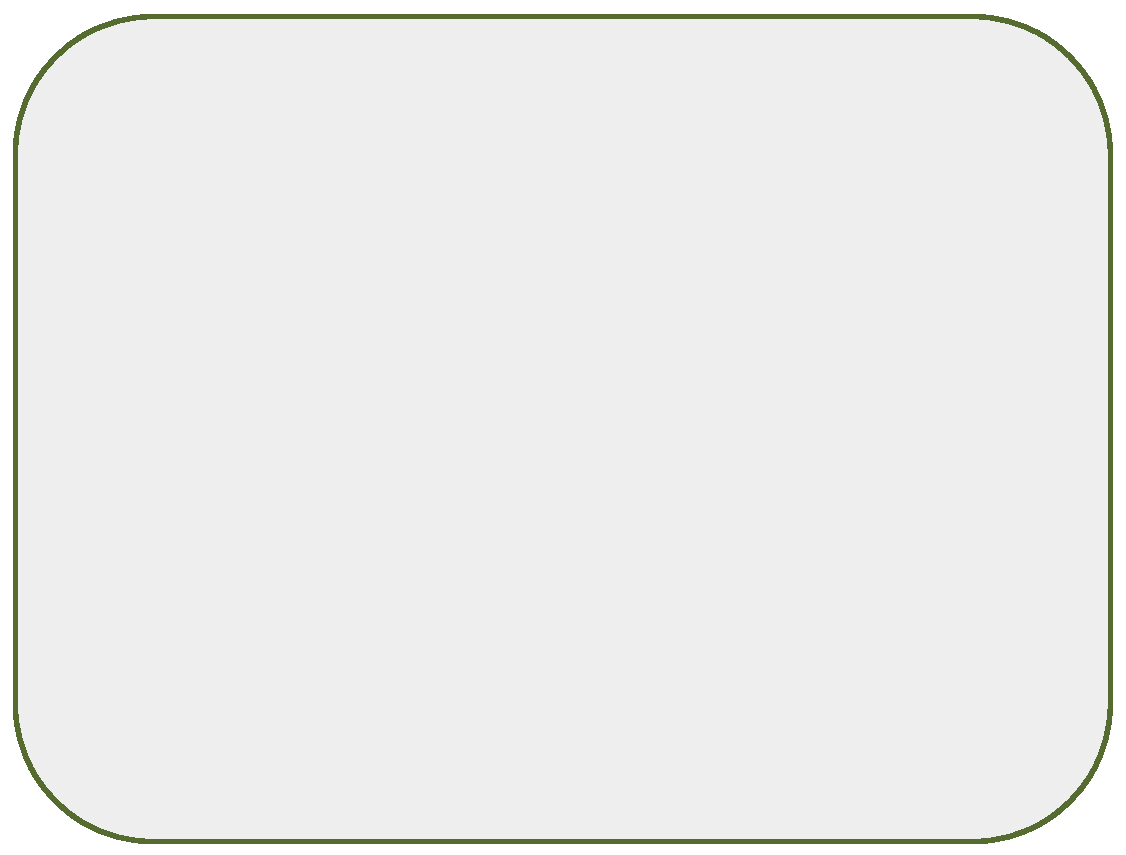
\includegraphics [width=0.8 \linewidth ]{pics/bg_33}%
		
	\end{textblock*}
	
	\begin{textblock*}{0.73\paperwidth}(0.05 \paperwidth, -19 mm)
		
	\begin{itemize}
		
		
		
		\item How to ?
		
	
			
			
		\end{itemize}
		
	
		
	\end{textblock*}
	
	
\end{frame}




\begin{frame}[allowframebreaks,plain]{References}

\begin{thebibliography}{99} % Beamer does not support BibTeX so references must be inserted manually as below


\appendix
\backupbegin

\footnotesize

\justifying 

\bibitem{omni}
Ya Su, Youjian Zhao, Chenhao Niu, Rong Liu, Wei Sun, and Dan Pei. 2019.
Robust anomaly detection for multivariate time series through stochastic recurrent
neural network. In SIGKDD. 2828–2837



\end{thebibliography}
\end{frame}

\begin{frame}[plain]{}
	\centering \huge
	\textbf{Thanks for your attention!}
\end{frame}









\backupend

\end{document} 


